\documentclass{article}

% Language setting
% Replace `english' with e.g. `spanish' to change the document language
\usepackage[english]{babel}

% Set page size and margins
% Replace `letterpaper' with `a4paper' for UK/EU standard size
\usepackage[letterpaper,top=1cm,bottom=1.5cm,left=2cm,right=2cm,marginparwidth=1.75cm]{geometry}

% Useful packages
\usepackage{amsmath}
\usepackage{graphicx}
\usepackage[colorlinks=true, allcolors=blue]{hyperref}

\title{Your Paper}
\author{You}

\begin{document}
\maketitle

\begin{abstract}
Your abstract.
\end{abstract}

\section{Introduction}

TODO


\section{Use-case 1}


Transformers have been used to encode proteins as vectors in a high-dimensional space, where sequences with similar properties are mapped closely together. This study~\cite{rives_biological_2021} demonstrates that after training, the representation space of a transformer model clusters orthologous genes effectively. This is visualized through t-SNE and PCA (figure~\ref{fig:gene-tsne}), which show that species and orthology become principal axes of variation, indicating that unsupervised learning captures biological variations. This learned structure allows for improved recovery of proteins based on biological properties using vector similarity queries, confirming that biological information is encoded within the representation space.
\begin{figure}[ht]
    \centering
    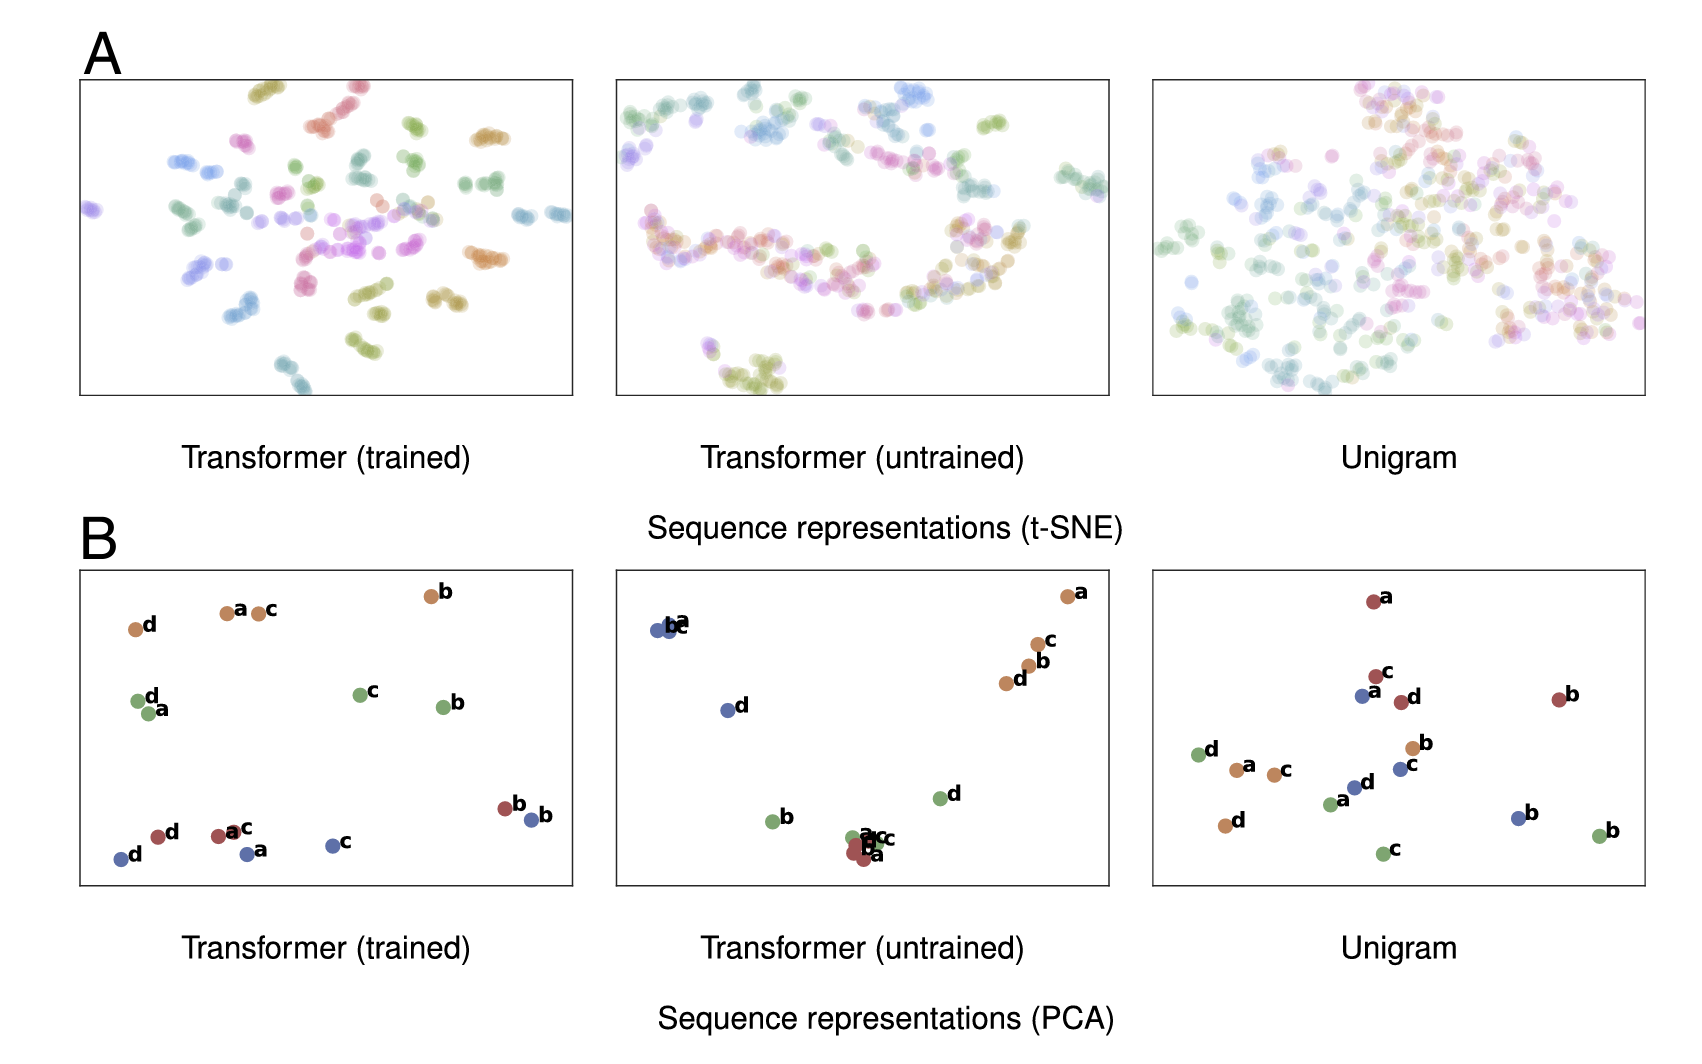
\includegraphics[width=0.8\linewidth]{img/gene-tsne.png}
    \caption{Enformer's analysis of a genetic variant (rs11644125 C/T) showing its impact on NLRC5 gene expression, with model predictions suggesting the T allele reduces expression, possibly through altered SP1 transcription factor binding, as validated by cap analysis gene expression (CAGE) data in peripheral blood mononuclear cells (PBMCs).}\label{fig:gene-tsne}
\end{figure}
    

\section{DNABERT}
DNABERT is a bidirectional encoder pre-trained on genomic DNA sequences with up- and downstream nucleotide contexts.
For short DNA sequences


\section{Enformers}
The Enformer model~\cite{avsec_effective_2021} utilizes transformer modules, known for their effectiveness in natural language processing, to analyze DNA sequences. Its key features include:
\begin{itemize}
    \item Transformer Layers: These enable the model to consider each part of the DNA sequence in relation to the entire sequence, crucial for integrating distant genomic elements.
    \item Extended Receptive Field: Enformer can analyze elements up to 100 kb from the transcription start site, much further than previous models, allowing it to capture a broader range of regulatory elements like distant enhancers.
    \item Attention Mechanism: This allows the model to weigh different parts of the sequence differently, depending on their relevance to gene expression.
\end{itemize}
By utilizing existing gene expression data, Enformer can be adapted to Dicty's genome, enabling predictions of gene expression levels based on genomic sequences.

\subsection{Effects of genetic variants}

Enformer is a computational model that can predict the effects of genetic variants on gene expression in a cell-type-specific manner, which is valuable for fine-mapping noncoding associations from genome-wide association studies (GWAS). Figure~\ref{fig:variant} depicts Enformer's predictive analysis of a genetic variant (rs11644125 C/T) showing its impact on NLRC5 gene expression, with model predictions suggesting the T allele reduces expression, possibly through altered SP1 transcription factor binding, as validated by cap analysis gene expression (CAGE) data in peripheral blood mononuclear cells (PBMCs).
\begin{figure}[ht]
\centering
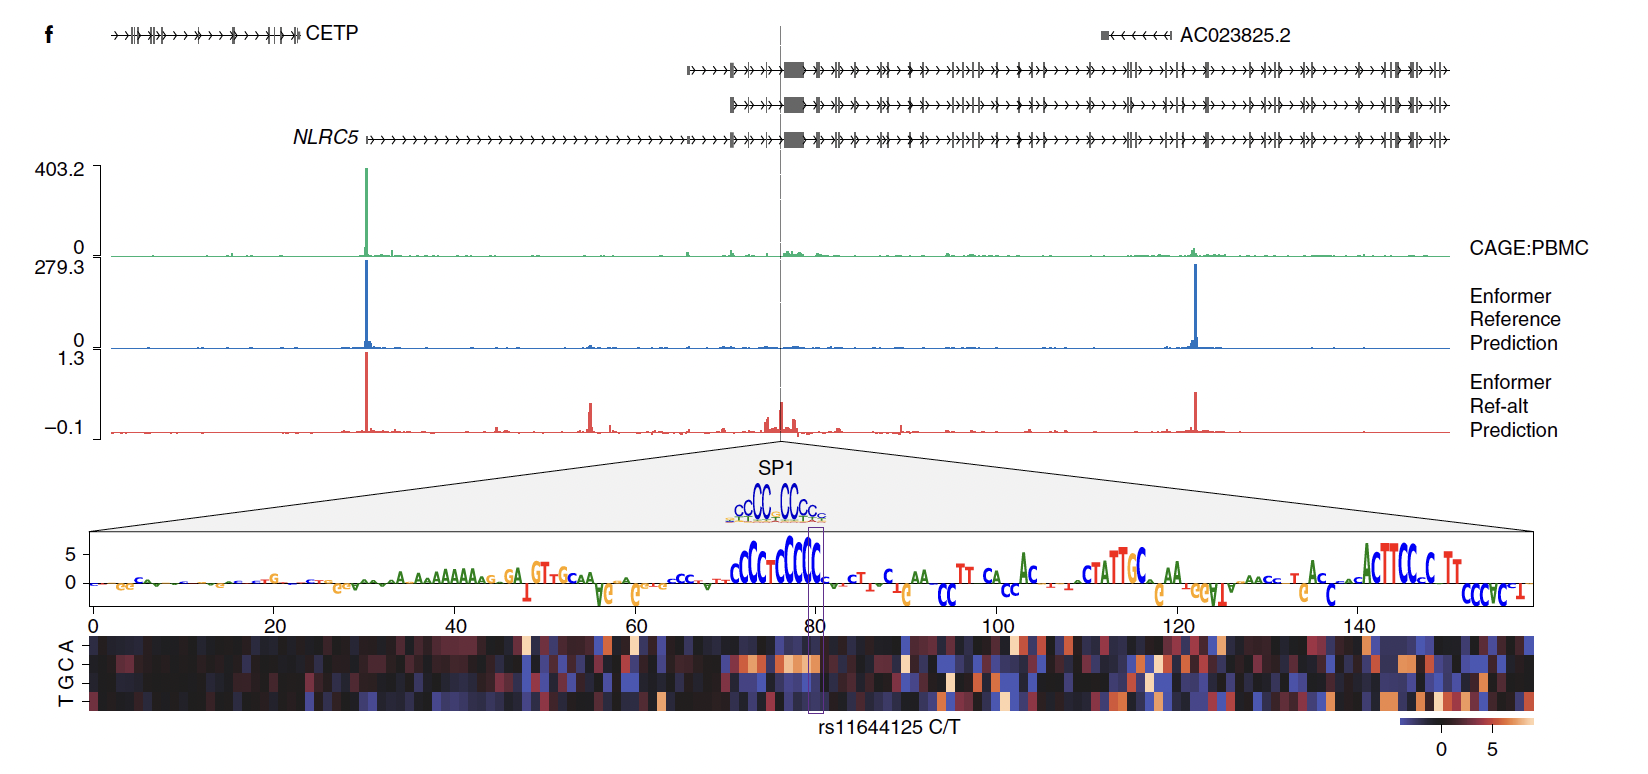
\includegraphics[width=0.8\linewidth]{img/variant.png}
\caption{Enformer's analysis of a genetic variant (rs11644125 C/T) showing its impact on NLRC5 gene expression, with model predictions suggesting the T allele reduces expression, possibly through altered SP1 transcription factor binding, as validated by cap analysis gene expression (CAGE) data in peripheral blood mononuclear cells (PBMCs).}\label{fig:variant}
\end{figure}

\bibliographystyle{unsrt}
\bibliography{sample}

\end{document}